% $Header$

\documentclass{beamer}
\usepackage{natbib,mathtools,tikz}
\usetikzlibrary[graphs]
\usetikzlibrary{decorations.markings}
% This file is a solution template for:

% - Talk at a conference/colloquium.
% - Talk length is about 20min.
% - Style is ornate.



% Copyright 2004 by Till Tantau <tantau@users.sourceforge.net>.
%
% In principle, this file can be redistributed and/or modified under
% the terms of the GNU Public License, version 2.
%
% However, this file is supposed to be a template to be modified
% for your own needs. For this reason, if you use this file as a
% template and not specifically distribute it as part of a another
% package/program, I grant the extra permission to freely copy and
% modify this file as you see fit and even to delete this copyright
% notice. 


\mode<presentation>
{
  \usetheme{Warsaw}
  % or ...

  \setbeamercovered{transparent}
  % or whatever (possibly just delete it)
}


\usepackage[english]{babel}
% or whatever

\usepackage[latin1]{inputenc}
% or whatever

\usepackage{times}
\usepackage[T1]{fontenc}
% Or whatever. Note that the encoding and the font should match. If T1
% does not look nice, try deleting the line with the fontenc.


\title[Ice anisotropy] % (optional, use only with long paper titles)
{Mesoscale anisotropic ice flow and stratigraphic disturbances}

%\subtitle
%{Include Only If Paper Has a Subtitle}

\author[Michael Hay] % (optional, use only with lots of authors)
{ 
  Mike Hay\inst{1}\\
  \footnotesize{
    Committee:\\
    Ed Waddington (advisor and chair),  Twit Conway, Gerard Roe, and Randy Leveque (GSR)\\
    Thanks to:\\
    Don Voigt, Joan Fitzpatrick, and Dan Kluskiewicz
    }
  }
% - Give the names in the same order as the appear in the paper.
% - Use the \inst{?} command only if the authors have different
%   affiliation.

\institute[University of Washington] % (optional, but mostly needed)
{
  \inst{1}%
  Department of Earth and Space Sciences\\
  University of Washington
  \and
  }
% - Use the \inst command only if there are several affiliations.
% - Keep it simple, no one is interested in your street address.

\date[CFP 2003] % (optional, should be abbreviation of conference name)
%{Conference on Fabulous Presentations, 2003}
% - Either use conference name or its abbreviation.
% - Not really informative to the audience, more for people (including
%   yourself) who are reading the slides online

\subject{Theoretical Computer Science}
% This is only inserted into the PDF information catalog. Can be left
% out. 



% If you have a file called "university-logo-filename.xxx", where xxx
% is a graphic format that can be processed by latex or pdflatex,
% resp., then you can add a logo as follows:

% \pgfdeclareimage[height=0.5cm]{university-logo}{university-logo-filename}
% \logo{\pgfuseimage{university-logo}}



% Delete this, if you do not want the table of contents to pop up at
% the beginning of each subsection:
%\AtBeginSubsection[]
%{
%  \begin{frame}<beamer>{Outline}
%    \tableofcontents[currentsection,currentsubsection]
%  \end{frame}
%}


% If you wish to uncover everything in a step-wise fashion, uncomment
% the following command: 

%\beamerdefaultoverlayspecification{<+->}


\begin{document}

\begin{frame}
  \titlepage
\end{frame}

\begin{frame}{Outline}
  \tableofcontents
  % You might wish to add the option [pausesections]
\end{frame}


% Structuring a talk is a difficult task and the following structure
% may not be suitable. Here are some rules that apply for this
% solution: 

% - Exactly two or three sections (other than the summary).
% - At *most* three subsections per section.
% - Talk about 30s to 2min per frame. So there should be between about
%   15 and 30 frames, all told.

% - A conference audience is likely to know very little of what you
%   are going to talk about. So *simplify*!
% - In a 20min talk, getting the main ideas across is hard
%   enough. Leave out details, even if it means being less precise than
%   you think necessary.
% - If you omit details that are vital to the proof/implementation,
%   just say so once. Everybody will be happy with that.

\section{Motivation}

\subsection{Strigraphic disturbances}

\begin{frame}{}{Subtitles are optional.}
  % - A title should summarize the slide in an understandable fashion
  %   for anyone how does not follow everything on the slide itself.

  \begin{itemize}
  \item
    
  \item
    Use very short sentences or short phrases.
  \end{itemize}
\end{frame}

\begin{frame}{Ice is very anisotropic}

  
  \begin{itemize}
  \item Ice deforms mostly be shear parallel to the basal plane.
  \item Other slip systems ~100x harder
    \item If ice grains are random, no problem.
    \pause \item But they usually aren't.
    \pause \item Grains rotate away from the axes of extension $\rightarrow$ bulk anisotropic plasticity
  \item This can cause bulk flow to be highly anisotropic.
  \end{itemize}
\end{frame}

\subsection{Different kinds of disturbances}

\subsection{Previous Work}

\begin{frame}{Observed statigraphic disturbances}
   \begin{columns}[T]
     \column{0.7\textwidth}
     \begin{itemize}
       \item There are smaller-scale disturbances seen well off beds.
       \pause $\rightarrow$ Too short wavelength to be due to bed.
     \end{itemize}
     \includegraphics[width=0.5\textheight]{stripes}
     \column{0.3\textwidth}
     \includegraphics[width=\textwidth]{z_fold}
     \end{columns}

\end{frame}


\section{Current work}

\subsection{Ice fabric evolution}

\begin{frame}{Introduction}
   \begin{itemize}
      \item \citet{azuma94} 
      \item \citet{thorsteinsson2002nni} developed a fabric model including nearest-neighbor interaction.
      \item We have developed a new model for evolution of a finite number of grains.
      \item The model includes generalized nearest neighbor interaction, mass conservation, and recrystallization.
   \end{itemize}
\end{frame}

\begin{frame}{Neighbors and mass balance}
   \begin{itemize}
      \item Each grain has a number of nearest neighbors in an undirected graph.
      \item Grains transfer mass between each other - one grain's loss is another's gain.
      \item Mass flux is determined by grain boundary velocity and shared boundary area.

   \end{itemize}
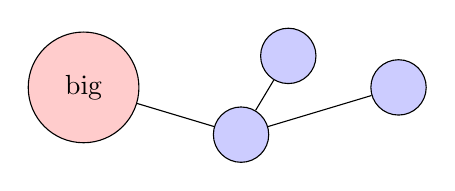
\begin{tikzpicture}[main_node/.style={circle,fill=blue!20,draw,minimum size=2em,inner sep=3pt]},scale=2]

    \node[circle,fill=red!20,draw,minimum size=4em] (1) at (0,0) {big};
    \node[main_node] (2) at (1, -0.3)  {};
    \node[main_node] (3) at (1.3, 0.2) {};
    \node[main_node] (4) at (2,0) {};
    \draw (1) -- (2) -- (3) -- (2) -- (4);
\end{tikzpicture} 
\end{frame}

\begin{frame}{Normal grain growth}
   \begin{itemize}
      \item Average grain size increases with depth, until polygonization and recrystallization become important.
      \item This is driven by curvature energy: Highly curved interfaces have a lot of free energy $\rightarrow$ small grains shrink
      \item Grain-boundary velocity computed by estimating the curvature at the interface.
   \end{itemize}



\begin{tikzpicture}[
    tangent/.style={
        decoration={
            markings,% switch on markings
            mark=
                at position #1
                with
                {
                    \coordinate (tangent point-\pgfkeysvalueof{/pgf/decoration/mark info/sequence number}) at (0pt,0pt);
                    \coordinate (tangent unit vector-\pgfkeysvalueof{/pgf/decoration/mark info/sequence number}) at (1,0pt);
                    \coordinate (tangent orthogonal unit vector-\pgfkeysvalueof{/pgf/decoration/mark info/sequence number}) at (0pt,1);
                }
        },
        postaction=decorate
    },
    use tangent/.style={
        shift=(tangent point-#1),
        x=(tangent unit vector-#1),
        y=(tangent orthogonal unit vector-#1)
    },
    use tangent/.default=1
]
\draw [
    tangent=0.6,
    tangent=0.8
] (0,0)
    to [out=50,in=120] (5,2)
    to [out=-60, in=110] (7,1);
%\draw [blue, thick, use tangent] (-3,0) -- (3,0);
\draw [orange, thick,->, use tangent=1] (0,0) -- (0,-1);
\draw [orange, thick,->, use tangent=2] (0,0) -- (0,1);
\end{tikzpicture}

\end{frame}


\subsection{Coupled anisotropic ice flow/fabric evolution}
\begin{frame}{Flow and fabric}
\begin{itemize}
   \item Ice fabric development is driven by flow, so this is a coupled system.
   \item \citet{montgomery-smith2011} found that Stokes flow of a fluid with slender fiber inclusions coupled to Jeffery's equation is unstable in response to perturbations of the orientation distribution function.
   \item \citet{gillet2006} found a large-scale Kelvin-Helmholtz-looking instability in their coupled model Jefferys/linear anisotropic ice flow model.
   \item Can an initial random perturbation become a strong perturbation?
\end{itemize}
\end{frame}
\begin{frame}{Shear bands and boudinage}
   \begin{columns}[T]
   \column{0.6\textwidth}
   \begin{itemize}
      \item Under horizontal simple shear, c-axes go to vertical - soft ice
      \item A layer that is initially softer will shear faster, and get softer faster 
      $\rightarrow$ a shear band.
      \item Boudinage is different. C-axes go to vertical with uniaxial compression, but that's the hard orientation.
   \end{itemize}
   \column{0.5\textwidth}
   \includegraphics[width=3in]{boudinage}
\end{columns}
\end{frame}

\begin{frame}{Layer folding}
   \begin{itemize}
      \item Shear overturns incipient wrinkles, horizontal extension flattens them.
      \item \citet{alley97} showed that anisotropy exacerbates this by making ice soft in shear and hard in uniaxial compression.
      \item Incipient wrinkles could be caused by stripes, or transient flow.
   \end{itemize}
\end{frame}

\begin{frame}{GOLF flow}
   \begin{columns}{T}
   \column{0.5\textwidth}
   \begin{itemize}
      \item The General Orthotropic Linear Flow (GOLF) law is a constitutive relation depending on six viscosity parameters.
      \item It assumes the ODF is orthotropic.
   \end{itemize}
   \column{0.5\textwidth}
   \begin{equation}
   S_{ij} = \eta_0 \left[ \eta_r M_{rkl} D_{kl} \left( M_{rij}^D \right)  + \eta_{r+3} \left( D_{ik} M_{rkj} + D_{kj} M_{rik} \right)^D \right],
   \end{equation}
\end{columns}
\end{frame}

\begin{frame}{Fabric evolution}
   %closure approx
   \begin{itemize}
      \item \citet{gillet2006} use a tensor-closure approximation for Jefferys equation. This very common in fiber injection molding modeling. 
      \item $A^2= < c \otimes c>$. 
   \end{itemize} \\
   \begin{equation}
      \frac{\partial A_{ij}}{\partial t} = -\frac{\partial}{\partial x_k} A_{ij} u_k + W_{ik} A_{kj} - A_{ik} W_{kj} - (D_{ik}W_{kj} + D_{kj}W_{ik}) + 2 \mathbb{A}_{ijkl} C_{kl}
   \end{equation}

\end{frame}

\begin{frame}{Perturbations}
\end{frame}

\begin{frame}{Other analytical work}
   \begin{itemize}
      \item Anisotropic ice flow is still a relatively untapped area.
      \item 
   \end{itemize}
\end{frame}

\section{Future work}

\begin{frame}{Is GOLF sufficient to explain anisotropic flow?}
   \begin{itemize}
      \item Fluids made up of linearly viscous transversely isotropic components do not depend on higher than $4^{th}$ order orientation tensors.
      \item GOLF assumes orthotropy, which does not hold in general for fourth order tensors.
      \item Also, ice is not linear, and nearest-neighber interactions seem to be important for ice.
      \item Does this mean that we need a more general flow model to address these shortcomings? \\
         \pause I don't think so, but maybe.
   \end{itemize}
\end{frame}
\begin{frame}{Is GOLF sufficient to explain anisotropic flow?}
   \begin{itemize}
      \item Nearest neighbor interaction makes a big difference with fabric evolution. Some grains get $>10 \times$ softness.
      \item This only makes for differences of $~1\%$ in bulk viscosity. But is is possible to construct fabrics where it the difference is bigger.
      \item Strain softening might be a similar situation.
      \item I propose investigating this question numerically for different fabrics. This will determine whether it is necessary to expand on GOLF.
      \item Prediction of fabric orientation would be improved by a higher-order evolution equation, either up to the sixth-order orientation tensor or using spherical harmonics.
   \end{itemize}
\end{frame}
\begin{frame}{Numerical flow modeling}
   \begin{itemize}
      \item To expand things beyond first order, I propose investigating mesoscale anisotropic flow with a 3d model in a box geometry.
      \item We can user Elmer/Ice FEM with the GOLF flow law.
      \item If we roll our own, we would use a simple finite volume scheme. Numerically, it is similar to to standard Stokes flow.
   \end{itemize}
\end{frame}

\begin{frame}{Summary}
   \begin{itemize}
      \item This provides a plan for three or four papers.
      \item We will submit the paper on the fabric model shortly.
      \item The  
   \end{itemize}
\end{frame}


% All of the following is optional and typically not needed. 
\appendix
\section<presentation>*{\appendixname}
\subsection<presentation>*{For Further Reading}

\begin{frame}[allowframebreaks]
  \frametitle<presentation>{References}
    
  %\beamertemplatebookbibitems
  % Start with overview books.
  \bibliographystyle{igs}
  \bibliography{anis}
\end{frame}

\end{document}


